\documentclass[a4paper,oneside,12pt]{book}
%----------------------------------------------------------------------------------------
%	WELCOME!
%   It's probably worth having a read through this file to set up the broad parameters.
%----------------------------------------------------------------------------------------

%----------------------------------------------------------------------------------------
%	COVER PAGE
%   The cover page is laid out in title/title.tex. You can choose a colour
%   or black and white logo
%----------------------------------------------------------------------------------------

%----------------------------------------------------------------------------------------
%	THESIS INFORMATION
%   Put title, author name, degree, type of work, school, department in here
%   It will be used for the title page and for the embedded PDF information
%----------------------------------------------------------------------------------------

\newcommand{\thesistitle}{An Investigation into Deep Reinforcement Learning in Atari 2600 Video Games} % Your thesis title, this is used in the title and abstract
\newcommand{\degree}{BAI (Computer Engineering)} % Your degree name, this is used in the title page and abstract
\newcommand{\typeofthesis}{Final Year Project} % dissertation, Final Year Project, report, etc.
\newcommand{\authorname}{Jack Cassidy} % Your name, this is used in the title page and PDF stuff
%% Comment out the next line if you don't want your ID to appear
\newcommand{\authorid}{14320816} % Your ID
\newcommand{\keywords}{machine learning, reinforcement learning} % Keywords for your thesis
\newcommand{\school}{\href{http://www.scss.tcd.ie}{School of Computer Science and Statistics}} % Your school's name and URL, this is used in the title page

%% Comment out the next line if you don't want a department to appear
%\newcommand{\department}{\href{http://recsearchgroup.university.com}{Department Name}} % Your research group's name and URL, this is used in the title page

\AtBeginDocument{
\hypersetup{pdftitle=\thesistitle} % Set the PDF's title to your title
\hypersetup{pdfauthor=\authorname} % Set the PDF's author to your name
\hypersetup{pdfkeywords=\keywords} % Set the PDF's keywords to your keywords
\hypersetup{pdfsubject=\degree} % Set the PDF's keywords to your keywords
}

%% Language and font encodings
\usepackage[T1]{fontenc} 
\usepackage[utf8]{inputenc}
\usepackage[english]{babel}

%% Bibliographical stuff
\usepackage{natbib}
%% Document size
% include showframe as an option if you want to see the boxes
\usepackage[a4paper,top=2.54cm,bottom=2.54cm,left=2.54cm,right=2.54cm,headheight=16pt]{geometry}
\usepackage{listings}
\usepackage{color}
\usepackage{longtable}
\definecolor{codegreen}{rgb}{0,0.6,0}
\definecolor{codegray}{rgb}{0.5,0.5,0.5}
\definecolor{codepurple}{rgb}{0.58,0,0.82}
\definecolor{backcolour}{rgb}{0.95,0.95,0.92}
 
\lstdefinestyle{mystyle}{
    backgroundcolor=\color{backcolour},   
    commentstyle=\color{codegreen},
    keywordstyle=\color{magenta},
    numberstyle=\tiny\color{codegray},
    stringstyle=\color{codepurple},
    basicstyle=\footnotesize,
    breakatwhitespace=false,         
    breaklines=true,                 
    captionpos=b,                    
    keepspaces=true,                 
    numbers=left,                    
    numbersep=5pt,                  
    showspaces=false,                
    showstringspaces=false,
    showtabs=false,                  
    tabsize=2
}
\lstset{style=mystyle}

%% Useful packages
\usepackage{amsmath}
% \numberwithin{equation}{section}
\usepackage[autostyle=true]{csquotes} % Required to generate language-dependent quotes in the bibliography
\usepackage[pdftex]{graphicx}
\usepackage{wrapfig}
\usepackage[colorlinks=true, allcolors=black]{hyperref}
\usepackage{caption} % if no caption, no colon
\usepackage{subcaption}
\usepackage{sfmath} %use sans-serif in the maths sections too
\usepackage[parfill]{parskip}    % Begin paragraphs with an empty line rather than an indent
\usepackage{setspace} % to permit one-and-a-half or double spacing
\usepackage{enumerate} % fancy enumerations like (i) (ii) or (a) (b) and suchlike
\usepackage{booktabs} % To thicken table lines
\usepackage{fancyhdr}
\usepackage{algorithm}
\usepackage{algpseudocode}
\usepackage{multicol}
\graphicspath{{images/}}
\pagestyle{plain} % Embrace simplicity!
\bibliographystyle{unsrtnat}
\setcitestyle{numbers,square}
%% The Mechanical engineers require your name and ID on the top of every page.
%% Uncomment the following block if you want your name and ID at the top of
%% (almost) every page.

%\pagestyle{fancy}
%\fancyhf{} % sets both header and footer to nothing
%\renewcommand{\headrulewidth}{0pt}
%\cfoot{\thepage}
%\ifdefined\authorid
%\chead{\it \authorname\ (\authorid)}
%\else
%\chead{\it \authorname}
%\fi
%% End of block

%% It is not a requirement of the university that the font should be sans-serif, but
%% the Mechanical engineers require it. Comment out the following line to disable it
\renewcommand{\familydefault}{\sfdefault} %use the sans-serif font as default
%% If you're not using sans-serif, consider using Palatino instead of the LaTeX standard
%\usepackage{mathpazo} % Use the Palatino font by default if you prefer it to Computer Modern

% \renewcommand{\theequation}{\arabic{equation}} %% use continuous equation numbers

%% Format Chapter headings appropriately
\usepackage{titlesec}
\titleformat{\chapter}[hang] 
{\normalfont\huge\bfseries}{\thechapter}{1cm}{} 

\title{\thesistitle}
\author{\authorname}

\frontmatter
\begin{document}
\begin{titlepage}

\center % Center everything on the page

%% All the text parameters should be taken from the start of the main.tex file.
%% You should only alter stuff here if you want to change the layout

%----------------------------------------------------------------------------------------
%	LOGO SECTION
%----------------------------------------------------------------------------------------
%% Choose one of the following -- a colour or black-and-white logo


\includegraphics{title/Trinity_RGB_transparent_main.png}\\[1cm] 
%
\includegraphics[width=12cm]{title/black-stacked-trinity.jpg}\\[1cm] 

\Large \school\\[1.5cm] % Minor heading such as course title
\ifdefined\department
\large \department\\[1.5cm] % Minor heading such as course title
\fi

%----------------------------------------------------------------------------------------
%	TITLE SECTION
%----------------------------------------------------------------------------------------
\makeatletter
{ \huge \bfseries \thesistitle}\\[1.5cm] % Title of your document
 

%----------------------------------------------------------------------------------------
%	AUTHOR SECTION
%----------------------------------------------------------------------------------------

\ifdefined\authorid
\authorname\\ % Your name
\authorid\\ % Your Student ID
Supervisor: Vincent Wade\\[2cm]
\else
\authorname\\[2cm] % Your name
\fi

%----------------------------------------------------------------------------------------
%	DATE SECTION
%----------------------------------------------------------------------------------------

{\large \today}\\[2cm] % Date, change the \today to a set date if you want to be precise

 
%----------------------------------------------------------------------------------------
%	TYPE OF THESIS SECTION
%----------------------------------------------------------------------------------------
 A \typeofthesis\ submitted in partial fulfilment\\of the requirements for the degree of BAI (Computer Engineering)

\vfill % Fill the rest of the page with whitespace

\end{titlepage}
\pagenumbering{roman}
\section*{\Huge{Declaration}}
\vspace{1cm}
I hereby declare that this project is entirely my own work and that it has not been submitted as an exercise for a degree at this or any other university.

\vspace{1cm}
I have read and I understand the plagiarism provisions in the General Regulations of the University Calendar for the current year, found at \url{http://www.tcd.ie/calendar}.
\vspace{1cm}

I have also completed the Online Tutorial on avoiding plagiarism `Ready Steady Write', located at
\url{http://tcd-ie.libguides.com/plagiarism/ready-steady-write}.
\vspace{3cm}

Signed:~\rule{5cm}{0.3pt}\hfill Date:~\rule{5cm}{0.3pt}

\chapter*{Abstract}
A short summary of the problem investigated, the approach taken and the key findings. This should be around 400 words, or less.

This should be on a separate page.

\newpage
\onehalfspacing\raggedright %\raggedright turns off justification and hypenation

\section*{\Huge{Acknowledgements}}
Thanks Mum!

You should acknowledge any help that you have received (for example from technical staff), or input provided by, for example, a company.
\tableofcontents
\listoffigures
\listoftables
\newpage
\section*{\Huge{Nomenclature}}
\begin{tabular}{lp{9cm}l}
    A        & Area of the wing                                                               & $m^{2}$ \\
    B                                                                                                   \\
    C        & Roman letters first, with capitals\ldots                                                 \\
    a        & then lower case.                                                                         \\
    b                                                                                                   \\
    c                                                                                                   \\
    $\Gamma$ & Followed by Greek capitals\ldots                                                         \\
    $\alpha$ & then lower case greek symbols.                                                           \\
    $\beta$                                                                                             \\
    $\epsilon$                                                                                          \\
    TLA      & Finally, three letter acronyms and other abbreviations arranged alphabetically           \\
\end{tabular}
\vspace{2cm}

If a parameter has a typical unit that is used throughout your report, then it should be included here on the right hand side.

If you have a very mathematical report, then you may wish to divide the nomenclature list into functions and variables, and then sub- and super-scripts.

Note that Roman mathematical symbols are typically in a serif font in italics.

\mainmatter
\chapter{Introduction}

\section{Motivation}
Machine Learning (ML) and Artificial Intelligence (AI) in 2018 are subjects that are almost unique in their ability to permeate into nearly every sphere, community and space in today's society. From the research community to the business world and the public eye through extensive media coverage, ML is on everyone's mind. Prolific engineer and business man, CEO of Tesla Motors and SpaceX, Elon Musk has publicly shared his views on Artificial Intelligence AI being the biggest existential threat to humanity and calls for increased regulation. % CITATION NEEDED??

Reinforcement Learning is a branch of ML, that perhaps receives less media attention but is nonetheless set to revolutionize the field of AI. 
\section{Objectives}

\section{Research Methods}

\section{Report Overview}

\chapter{Figures, Tables and Referencing}
sIt is very important to properly refer in the text to any figures, tables or previously published work that you are discussing. Adequate and consistent referencing is one of the criteria which will be used to assess your project report.

\section{Figures}
Graphs, pictures and other images should be included in your report as a numbered, captioned figure. An example is given in Figure \ref{veldis}.

%%%%%%%%%%%%%%%%%%%%%%%%%%%%%%%%%%%%%%%%
\begin{figure}[h]
	\centering
	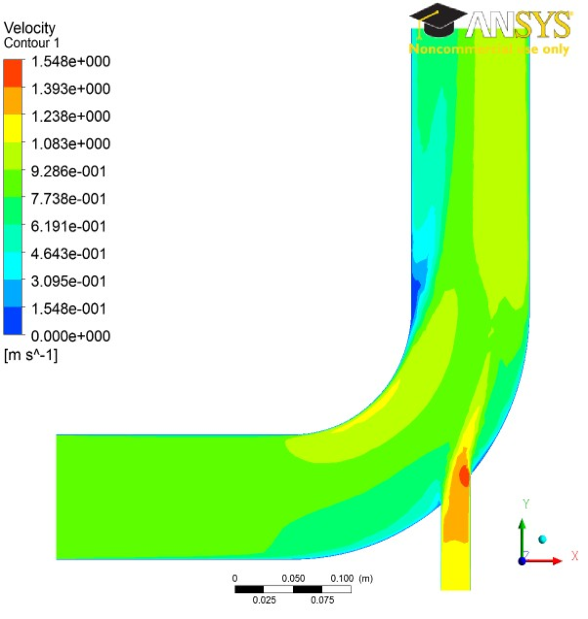
\includegraphics{background/5e1-1.pdf}
	\caption{Velocity distribution on the mid-plane for an inlet velocity for case 1.}
	\label{veldis}
\end{figure}
%%%%%%%%%%%%%%%%%%%%%%%%%%%%%%%%%%%%%%%%

The figure and caption should be centred. The figure numbering starts at 1 at the beginning of each chapter. The caption should provide a brief description of what is being shown. The figure should appear in the document after it is referred to in the text. No figure should be included which is not referred to in the text. Ensure that the size and resolution of images imported from software are sufficient to read any text.

\section{Tables}
Tables are an important way of displaying your results; Table \ref{tab:treatments} is a sample table, adapted from the Master/Doctoral Thesis template at \url{http://www.latextemplates.com/cat/theses}, which was generated with this code:

{\footnotesize
	\begin{verbatim}
\begin{table}[b]
\caption{The effects of treatments X and Y on the four groups studied.}
\label{tab:treatments}
\centering
\begin{tabular}{l l l}
\toprule
\textbf{Groups} & \textbf{Treatment X} & \textbf{Treatment Y} \\\midrule
1 & 0.2 & 0.8\\
2 & 0.17 & 0.7\\
3 & 0.24 & 0.75\\
4 & 0.68 & 0.3\\
\bottomrule\\
\end{tabular}
\end{table}
	\end{verbatim}
}

\begin{table}[b]
	\caption{The effects of treatments X and Y on the four groups studied.}
	\label{tab:treatments}
	\centering
	\begin{tabular}{l l l}
		\toprule
		\textbf{Groups} & \textbf{Treatment X} & \textbf{Treatment Y} \\
		\midrule
		1               & 0.2                  & 0.8                  \\
		2               & 0.17                 & 0.7                  \\
		3               & 0.24                 & 0.75                 \\
		4               & 0.68                 & 0.3                  \\
		\bottomrule\\
	\end{tabular}
\end{table}

Tables are numbered in the same way as figures. Typically tables also have a short caption, but this is not universally true. The number and caption appear above the table, not below as with figures. Again, no table should appear in the report which has not been referred to in the text. Tables should come after they are discussed in the text. The exact formatting of the table depends somewhat on the content of the table, but in general, the text in the table should be the same font and size as the main text. 

\section{Equations}
All equations should be numbered sequentially. Do not restart the numbering at the beginning of each chapter. Unlike figures and tables, you may not need to refer to every equation in the text. You should take care to format equations properly. Do no simply try to use plain text. Use the equation layout facilities. An example of how equations should appear is shown in Equation \ref{sampleequation}. Here is the code for it:

{\footnotesize
	\begin{verbatim}
\begin{equation}
\textrm{div}(\underline{u}) = \frac{\delta u}{\delta x} + \frac{\delta v}{\delta y} +
        \frac{\delta w}{\delta z} = 0
\label{sampleequation}
\end{equation} 
	\end{verbatim}
}

\begin{equation}
	\textrm{div}(\underline{u}) = \frac{\delta u}{\delta x} + \frac{\delta v}{\delta y} + \frac{\delta w}{\delta z} = 0
	\label{sampleequation}
\end{equation} 

\section{Referencing published work}
It is important to give appropriate credit to other people for the work that they have shared through publications. In fact, you must sign a declaration in your report stating that you understand the nature of plagiarism. As well as avoiding plagiarism, citing results or data from the literature can strengthen your argument, provide a favourable comparison for your results, or even demonstrate how superior your work is.

There are many styles to reference published work. For example, the parenthetical style (which is also called the Harvard style) uses the author and date of publication (e.g. ``Smith and Jones, 2001''). There is also the Vancouver (or the citation sequence) style, which is shown in this document. In the Vancouver style, the publications are cited using a bracket number which refers to the list in the References section at the end of the report. The references are listed in order that they are cited in the report. A variant is name sequence style in which the publications are referenced by number, but the list is arranged alphabetically. For example, the text might say: several studies have examined the sound field around tandem cylinders generated by flow\cite{fitzpatrick2003flow,finnegan2010experimental}, while other investigations have focused on the effect of an applied sound field on the flow\cite{hall2003vortex}. Papers from conference proceedings\cite{jordan2001array}, books\cite{paidoussis2010fluid} and technical reports\cite{reyes2007power,iea2011} can be dealt with in the same style.

The Vancouver style has the advantage that it is a little more compact in the text and does not distract from the flow of the sentence if there are a lot of citations. However, it has the disadvantage that it is not immediately clear to the reader what particular work has been referenced.

It actually does not matter which particular referencing style is used as long as three important considerations are observed:
\begin{itemize}
	\item the referencing style used throughout the document is consistent;
	\item all material used or discussed in the text is properly cited;
	\item nothing is included in the reference list that has not been cited.
\end{itemize}

This template has a suitable referencing style already set up -- you should use it and use the built-in BibTeX system to manage your references. See above for examples of how to cite a reference and look in the \texttt{sample.bib} file to see BibTeX references. Remember \href{http://scholar.google.com}{Google Scholar} and other search engines will give you BibTeX references for lots of academic publications. Otherwise, you can easily make up your own based on the examples in that file.

\chapter{State of the Art}
The current state of the field of RL is vast. More and more it is being utilized as the next step towards more efficient and intelligent ML systems (\citet{survey-drl}). This section will be divided into two discussions. The first will give a basic survey of the types of different applications of RL today. The second section will discuss the state of the art for RL research within the video game test bed.

\section{Robotics}
Robotics is a field very suited to RL techniques. It closely follows the basic definition of an RL task involving an agent exploring an environment through trial and error to maximize some reward function. Although it is well suited, there are many challenges that face RL techniques in robotics. The recent work of (\citet{a3c}), the A3C algorithm (see subsequent section for an explanation of the algorithm), is an example of state of the art RL techniques addressing one of the most pressing issues for RL in robotics: the 'curse of dimensionality' with respect to the navigation of a robot through a complex environment. Coincidentally A3C has provided state of the art results in video game AI agent research results. \paragraph{}

The representation of state in robotics is often imperfect and noisy due to it's high levels of dimensionality and the resolution reduction of continuous physical measurements to discrete digital computer/controller representations. A mechanical representation of state such as robot limb position, or any other physical measurement usually have up to 6 DOF. In addition to state complexity, the action space in contrast to the Atari domain which is fixed and simple, can reach high dimensionality due to multiple DOF and the hardware complexity of most modern robots, where there can be a large number of motors and other components working in tandem, each adding to the complexity of the total action space. \paragraph{}

With respect to a robot that navigates through a complex, partially observable environment with dynamic obstacles, in addition to the high dimensional state size, the memory efficiency of remembering past experiences becomes a pressing issue as it is of utmost importance for a robot learning to navigate to be able to utilize past experiences to map its surroundings. A3C abandons experience replay in favour of a stacked Long Short Term Memory (LSTM) network running multiple agents that are exploring the environment in parallel, providing a wider range of experiences that scales with the number of parallel agents employed. This dramatically increased the memory efficiency of the implementation.

\section{Natural Language Processing}
Deep learning, more so than DRL, has been permeating into the field of Natural Language Processing (NLP). There have been many exciting revelations in NLP in recent years that interface with users regularly, such as chat bots, text prediction and machine translation (MT) etc. \paragraph{}

MT is simply defined as the sub-field of computer linguistics that investigates the use of software to translate text or speech from one language to another. The ability for systems to recognize full phrases and sentences and translate those accurately instead of simply substituting words is what defines good MT systems from others, as the latter will almost always be rife with grammatical errors in the target language. Neural Machine Translation (NMT) introduces deep learning into the MT sphere, to further the ability to recognize phrases and sentences. Recurrent neural networks (RNNs) are popular in NTM systems, owing to their internal memory which is suited to picking out patterns and phrases, as opposed to fully feed forward networks with no concept of internal remembrance. The basic architecture involves two RNN's, an encoding layer at the input sentence and a decoding layer at the translated sentence output. \paragraph{}

The current state of the art in NMT is Google's Neural Machine Translation (GNMT) system \citet{wu2016google}. It tackles the issues of speed of translation/inference, robustness in the face of translating sentences containing 'rare' words and incomplete translations. These are three issues that have \textit{severely} hampered the deployment of MT systems into production. The network architecture consists of an LSTM encoder with 8 layers and the same at the output. The residual connections between layers in the encoder and decoder, to introduce parallelism, and low-precision arithmetic during inference computations are used to tackle the speed of translation problem. Breaking up words into sub-word units or 'wordpieces' reduces the chances of finding 'rare' words by translating on sections rather than full words, but provides a balance of compute time over single character scale translation. Finally, a beam search technique to tackle the issue of incomplete translations. With these three features, GNMT has proved itself as a state of the art for MT and is in fact used in production at Google today.

\section{Deep Reinforcement Learning}
\subsection{Improvements to Deep Q-Network}
In 2013, the DQN breakthrough was the state of the art. Since then, many improvements and adaptations have been made on this algorithm, by DeepMind and other research groups. Such examples include the Double Q-Network adaptation (\citet{doubleq}) and the Dueling Q-network architecture (\citet{dueling}). Experience replay and target networks were two techniques added to the original architecture by DeepMind to add more stability to the learning process. Prioritized experience replay was then built on from experienced replay providing even better performance.

\subsubsection{Experience Replay and Target Network}
Instead of learning from the immediately previous experience when training the network, a large memory of past experiences are stored as tuples of $(s_t, a_t, r_{t}, s_{t+1}, term)$, where $term$ is a boolean indicating if this state transition was terminal (a gameover). The network is then trained from a random sampling of past experiences from this replay memory. It was found to greatly reduce the number of interactions the agent needed to have with the environment. However, this technique \textit{is somewhat} limited as there is no way to differentiate important experiences from unimportant ones. \paragraph{}

The target network is a secondary network $\hat{Q}$ cloned from the online Q-network $Q$, that is used to predict the targets $y_i$ when training $Q$. The weights of $\hat{Q}$ are cloned from $Q$ every $\tau$ training steps. This modification makes the algorithm more stable, as an increase to $Q(s_t, a_t)$ was often found to also increase $Q(s_{t+1}, a)$ for all $a$, thus also increasing the targets $y_i$. This can create a diverging solution in some cases. Freezing the weights makes the updates to $Q$ and the targets $y$ further apart, decreasing the likelihood of divergence (\citet{human}). \paragraph{}

\begin{algorithm}
    \caption{Deep Q-Network Algorithm with Experience Replay and a Target Network}\label{alg:DQN}
    \begin{algorithmic}[1]
        \State Initialize replay memory $D$ to capacity $N$
        \State Initialize $Q$ with random weights $\theta$
        \State Initialize $\hat{Q}$ with weights $\theta^-$ cloned from $\theta$
        \For{episode = 1, M}
        \State Initialize arbitrary first sequence of frames for initial state
        \For{t = 1, T}
        \State With probability $\epsilon$ select a random action $a_t$, otherwise select $a_t = max_a Q(s_t, a)$
        \State Execute action $a_t$ and observe reward $r_t$ and state $s_{t+1}$
        \State Store state transition $(s_t, a_t, r_t, s_{t+1}, term)$ in $D$
        \State Sample random mini batch $(s_i, a_i, r_i, s_{i + 1}, term)$ from $D$
        \If{$term = true$}
        \State Set $y_i = r_i$
        \Else
        \State Set $y_i = r_i + \gamma max_a Q(s_{i+1}, a)$ \label{DQN:target}
        \EndIf
        \EndFor
        \State Perform a gradient descent step on $(y_i - Q(s_i, a_i))^2$
        \If{$t$ is a multiple of $\tau$}
        $\theta^- \leftarrow \theta$
        \EndIf
        \EndFor
    \end{algorithmic}
\end{algorithm}

\subsubsection{Double Deep Q-Network}
In the standard Deep Q-Network algorithm \algref{alg:DQN}{DQN:target}, when training we use the same Q-Value to select and evaluate an action for the target $y$. This can result in overoptimistic Q-value estimates over time, leading to sub-optimal policies as certain actions are erroneously favoured over others due to early over estimations. Double Deep Q-Network (\citet{doubleq}) separates action selection from action evaluation in the target $y$. The online network $Q$ still estimates the best action to take based on a max operator on it's predicted vector of Q-values. We reuse the target network to then evaluate the effectiveness of this action. The updated target equation is given as:

\begin{align}
    \label{equ:DubTarget}
    y_i = r + \gamma \hat{Q}(s_{i+1}, argmax_aQ(s_{i+1}, a))
\end{align}

As with the original target network optimisation, the weights from $Q$ are copied to $\hat{Q}$
every $\tau$ training updates.

\begin{algorithm}
    \caption{Double Deep Q-Network Algorithm} \label{alg:DDQN}
    \begin{algorithmic}[1]
        \State Initialize replay memory $D$ to capacity $N$
        \State Initialize $Q$ with random weights $\theta$
        \State Initialize $\hat{Q}$ with weights $\theta^-$ cloned from $\theta$
        \For{episode = 1, M}
        \State Initialize arbitrary first sequence of frames for initial state
        \For{t = 1, T}
        \State With probability $\epsilon$ select a random action $a_t$, otherwise select $a_t = max_a Q(s_t, a)$
        \State Execute action $a_t$ and observe reward $r_t$ and state $s_{t+1}$
        \State Store state transition $(s_t, a_t, r_t, s_{t+1}, term)$ in $D$
        \State Sample random mini batch $(s_i, a_i, r_i, s_{i + 1}, term)$ from $D$
        \If{$term = true$}
        \State Set $y_i = r_i$
        \Else
        \State Set $y_i = r_i + \gamma \hat{Q}(s_{i+1}, argmax_aQ(s_{i+1}, a))$ \label{DDQN:target}
        \EndIf
        \EndFor
        \State Perform a gradient descent step on $(y_i - Q(s_i, a_i))^2$
        \If{$t$ is a multiple of $\tau$}
        $\theta^- \leftarrow \theta$
        \EndIf
        \EndFor
    \end{algorithmic}
\end{algorithm}

\subsection{Current State of the Art for Deep Q-Network}
\subsubsection{Dueling Q-Network Architecture}
The Dueling Q-Network Architecture is an improvement on the original Deep Q-Network's single stream, convolutional network into a single fully connected layer network architecture. It \textit{does not} provide any change to the underlying algorithms at work. For this reason, it can be applied to other RL algorithms that use Q-Values. The single stream fully connected layer is separated into two streams. One stream estimates the state value functions $V(s)$ and the other estimates a new function, the action advantage function $A(s, a)$.

\begin{align}
    \label{eq:adv}
    A(s, a) =  Q(s, a) - V(s)
\end{align}

The two streams are aggregated at the final layer to output $Q(s, a)$. The convolutional network in the upper half remains unchanged. $V(s)$ and $Q(s, a)$ we have explained the intuition for previously. The action advantage function $A(s, a)$ gives a relative importance of each action in a given state. Hence, the dueling architecture can learn which states are valuable separately from the effect of each action in each state. \paragraph{}

\begin{figure}[h]
    \centering
    \includegraphics[scale=0.35]{dueling_q}
    \caption{The original Deep Q-Network (above) vs. Dueling Q-Network (below) architecture (\citet{dueling})}
\end{figure}

The aggregating layer is not a simple sum of $A(s, a)$ and $V(s)$. It was found that equation \ref{eq:adv} ``is unidentifiable in the sense that given $Q$ we cannot recover $V$ and $A$ uniquely'' (\citet{dueling}). Instead we use a slightly augmented version:

\begin{align}
    Q(s, a) = V(s, a) + (A(s, a) - max_{a'} A(s, a'))
\end{align}

\subsubsection{Prioritized Experience Replay}
In regular experience replay, transitions are sampled randomly and uniformly from the replay memory collection, with no regard to which transitions the agent might learn more from at any given time. Prioritized experience replay was first suggested by (\citet{prioritized}) as a way to improve the efficiency of regular experience replay by replaying more important transitions more frequently. It is difficult to quantify the importance, or potential learning progress an agent can expect by replaying a transition, hence a reasonable estimation can be made to approximate it. (\citet{prioritized}) approximate learning progress with the magnitude of the TDE of a transition, a suitable value as many RL algorithms use TDE, including Q-Learning. Along with the tuple $(s_t, a_t, r_{t}, s_{t+1}, term)$, the TDE, $\delta$ is now also stored with each state transition. The TDE of each transition is updated after being sampled to prevent the highest rank transition from always being sampled. \paragraph{}

A greedy prioritization, where the maximum TDE experiences are always sampled is flawed. Transitions that first occur with a low TDE will effectively never be revisited. The same small set of experiences are repeatedly sampled, with such a lack of diversity the neural network is likely to overfit. To overcome this (\citet{prioritized}) propose a stochastic prioritization policy with two variants.
\begin{gather}
    \label{equ:prob_exp}
    P(i) = \frac{p_i^\alpha}{\sum_kp_k^\alpha} \\
    \label{equ:priority1}
    p(i) = |\delta_i| + \epsilon \\
    \label{equ:priority2}
    p(i) = \frac{1}{rank(i)}
\end{gather}
Where $P(i)$ is the probability of sampling transition $i$, $k$ is the number of transitions in the replay memory, $p(i)$ is the priority of transition $i$ and it's two variants are shown. Variant 1 is similar to a greedy prioritization, but $\epsilon$ prevents 0 TDE transitions from never being sampled. Variant 2 is based on $rank$, where $rank(i)$ is the rank of transition $i$ over all transitions when sorted by $|\delta|$.

\section{Video Games}

\subsection{A3C}
The team at DeepMind, in (\citet{a3c}) propose a new framework for training DRL agents. Multiple copies of the same agent are run asynchronously on a separate thread, all performing gradient descent updates to a single common neural network. At any given time, every agent will likely be experiencing a different state, giving a much greater view of the environment. This helps to mitigate the exploration vs. exploitation dilemma previously discussed. The framework, which we will refer to as 'asynchronous methods,' can be used to augment many different pre-existing DRL algorithms to improve their performance. As well as performance improvements, this framework significantly cuts the time to train an agent in the Atari 2600 test bed and can be accomplished on a standard multi-core CPU, as opposed to previous methods that have used specialized, expensive, GPU hardware. The results obtained in (\citet{a3c}) from their experiments were carried out on an unspecified 16-core CPU and an Nvidia K40 GPU. At the time of writing, an AMD Ryzen 1950X 16-core CPU costs \$874 and an Nvidia K40 costs \$2300 (prices from \texttt{www.amazon.com}). Thus asynchronous methods further lowers the economic barrier to entry to DRL. \paragraph{}

\begin{figure}[H]
    \centering
    \includegraphics[scale=0.5]{a3c}
    \caption{High level overview of Asynchronous Methods, (\citet{a3cimage})}
\end{figure}

Of the four augmented algorithms tested in (\citet{a3c}), Asynchronous Advantage Actor-Critic (A3C) stands as the current state of the art algorithm for training DRL agents. It performs better than all other competitors, including the most recent revisions of Deep Q-Network, in the Atari 2600 test bed in terms of game score, and in half the time of the previous state of the art. Additionally, DeepMind applied A3C to an interesting problem outside of the video game domain. An AI agent was taught to navigate the 3D maze environment Labyrinth, collecting rewards. The collectables were apples - worth 1 point and portals - worth 10 points. The agent was placed in a randomly generated maze each episode and was given 60 seconds to accumulate as much reward as possible. The agent peaked with an average score of 50, indicating that it had learned a general strategy for exploring randomised environments. The applications of this feat to fields such as robotics is exciting.

\subsection{Games of Imperfect Information}
Games of imperfect information mean that the player is unaware of the state or actions chosen by the opposite player. Games of imperfect information include Texas Hold'Em Poker, as players do not know the other player's card and Real-time strategy (RTS) games, as players cannot see the areas of the map where the other players are until they explore those areas. These scenarios provide new challenges for training more intelligent AI agents.

\subsubsection{Case Study: StarCraft 2 Learning Environment}
The StarCraft 2 Learning Environment (SC2LE) is a platform for testing RL AI agents in the game StarCraft 2, an RTS of imperfect information (\citet{starcraft}). It was created by DeepMind in collaboration with Blizzard Entertainment, the creators of StarCraft 2. The game is exceedingly more complex than the Atari 2600 games we have discussed previously.
\begin{itemize}
    \item Modern graphics. StarCraft 2 is a modern 3D game with a movable isometric camera perspective. This makes representing observations as a stack of game frames very difficult, as the pixel counts are high and parallax error is introduced.
    \item  Action space. The diversity of actions in StarCraft 2 is far higher, with approximately $10^8$ possibilities in a point-and-click fashion. Many actions require a sequence of primitive actions such as, drag box around units, select building to build, place building on map. The player can be controlling potentially hundreds of units of many different types and abilities, as well as having to manage resources, building and ensure the opposing players aren't attacking.
    \item Multiple agents. There can be up to 4 players in one game, all competing against one another for map control. This is a stark contrast to the single player Atari 2600 games competing against a single built-in game AI.
    \item Imperfect information. There is a 'fog-of-war' element that hides parts of the map the player does not actively have units in.
    \item Delayed rewards. The action of building a number of units, exploring an area of the map etc. can have rewards that do not materialize for many, many time steps. This provides a new frontier for agents capable of creating long term strategy.
\end{itemize}

\begin{figure}[H]
    \centering
    \includegraphics[scale=0.5]{sc2le}
    \caption{SC2LE interacting with an AI agent (\citet{starcraft})}
\end{figure}

For a more complete breakdown of the complexity of StarCraft 2, we refer the reader to the paper (\citet{starcraft}), specifically section 3.2. \paragraph{}

SC2LE provides a high level Python API for programmatic interaction with StarCraft 2, called PySC2 that has been optimized for training RL agents. To tackle the aforementioned problem of high dimensional 3D game graphics, PySC2 abstracts away the game's graphics and replaces them with feature layers, primitive shape objects representing more complex in-game objects, while still maintaining some spacial aspects.

\begin{figure}[H]
    \centering
    \includegraphics[scale=0.6]{pysc2}
    \caption{The feature layers of PySC2 (\citet{starcraft})}
\end{figure}

In the figure above, on the left side, we can see a specific type of attack unit being represented as the green circles, resources as grey circles, worker units as small red circles etc. On the right side are different representations of features available from the full resolution mini-map, including height (top left), visibility (second from top left) and unit hit points or lives (bottom right). \paragraph{}

SC2LE provides a set of 'mini-games,' which are stripped down versions of the original game intended to be much simpler scenarios, focused on obtaining a more fine grained objective. This allows training agents in progressive steps, building up to the ability to play a full game against multiple players. \paragraph{}

A set of benchmark results were published by (\citet{starcraft}) with the release of SC2LE. These results were obtained by a DeepMind RL agent trained using the A3C algorithm under 3 different network architectures. Although the results were underwhelming - the agent did not win a single game against the easiest built-in game AI, the fully convolutional network managed to utilize one of the unit's (Teran worker) abilities to move buildings out of attack range, thus managing a draw by surviving past the 30 minute time limit. However, no agent managed to devise a winning strategy. The ability to devise such an agent is still an open question.

\subsection{Performance Metrics} \label{subsec:metrics}
The most popular, general performance metrics used in (\citet{doubleq,dueling,deepmind1,human,a3c}) when evaluating algorithm performance on the Atari 2600 test bed are listed below.

\begin{itemize}
    \item Game score, the range of which will vary greatly between different games.
    \item Max Q-Value estimates
    \item Number of game frames survived
\end{itemize}

These metrics are gathered by running a predetermined number of evaluation games; where the agent selects it's action from the trained network. They are usually presented as a mean average, however there is an argument for taking the median value to lessen the effect of outliers (\citet{ale-eval-plat}). The evaluation runs are held after a regular number of training updates, where the agent solely exploits the trained policy and no learning updates take place. These intervals vary between different papers.

\subsubsection{Normalizing Scores}
The scales for scoring between two games can vary greatly, which makes it difficult to compare the performance of an algorithm on different games by quoting score alone. (\citet{ale-eval-plat}) recommend using normalizing all scores using predetermined reference values.

\begin{align}
    z_{g, i} = \frac{s_{g, i} - r_{g, min}}{r_{g, max} - r_{g, min}}
\end{align}

Where $z_{g, i}$ is the normalized score $s_i$ in game $g$. $[r_{g, min}, r_{g, max}]$ are reference values that we normalize to. These could be the minimum and maximum obtainable scores in the game, or more interestingly (\citet{human}) propose normalizing scores to the score achieved by a human player, where $r_{g, min} = \text{random players score} \text{and} r_{g, max} = \text{human players score}$. We can then see the algorithms percentage performance over human level. \paragraph{}

Average reward (normalized or not) and average frames survived are an interesting duo of performance metrics. Together, they can give a better understanding of \textit{what} the agent is learning to do. In some games, the score might be dependant on surviving for a long time, for others it might be to shoot as many 'things' as possible and rack up points.

\chapter{Design}
One of the primary objectives of this project is to build a system for comparing the performance of DRL algorithms when applied to agents in the Atari 2600 video game test bed. This chapter discusses the design and implementation of that system. \paragraph{}

We begin with a discussion of the different platforms and tools available to us to aid in the implementation. We will not be building the system completely from scratch, we will require an emulator to host our agents and environments and external libraries to prevent 'reinventing the wheel' when it comes to the programming of the system. We will follow with a broad system overview and then an in-depth look at the system architecture. It is the aim of these sections to leave the reader with a thorough understanding of exactly \textit{how} the system operates. Finally we will close with the reasoning behind the choice of games, Space Invaders and Breakout, and algorithms, Deep Q-Network (DQN), Double Deep Q-Network (2DQN) and Dueling Double Deep Q-Network (3DQN), for the evaluation of our system.

\section{Platform and Tool Choices}
\subsection{OpenAI Gym and The ALE}
The OpenAI Gym and the ALE were introduced in Chapter 2 as RL research tools for the video game domain. Here we give the strengths (+) and weaknesses (-) of each, and the reasoning behind the selection of the ALE as the foundation of our system.

\textbf{OpenAI Gym}
\begin{itemize}
    \item[$+$] Provides a great diversity of environments.
    \item[$+$] The high-level API is simple to use.
    \item[$-$] The high-level API does not provide enough control nor is it as feature rich as the ALE.
    \item[$-$] The selection of Atari 2600 environments is limited.
\end{itemize}

\textbf{The ALE}
\begin{itemize}
    \item[$+$] Provides a large range of supported Atari 2600 environments (61, see \ref{app:ALE_Games} for full list) with more planned for the future.
    \item[$+$] Many more features and higher level of control, as detailed in Chapter 2.
    \item[$-$] The Python wrapper is slightly behind the C++ API.
    \item[$-$] The environments are limited to Atari 2600.
\end{itemize}

Having weighed the strengths and weaknesses of both tools, it became clear that the low-level amount of control that the ALE provides would be imperative for the implementation of the system, in terms of customization and data collection. The suite of Atari 2600 environments is a well known test bed for RL research, hence the additional environments provided by the OpenAI Gym were not needed.

\subsection{Choice of Programming Languages and Libraries}
\subsubsection{Python}
Python is a high level programming language, made popular by it's simplistic human-readable syntax, it's ability to perform tasks in minimal lines of code, and it's vast community support in the form of modules (Python syntax for external libraries) \cite{python}. Python 3.5 was used to build the system in it's entirety. It is the default language to use when implementing deep neural networks thanks to the wide support of deep learning modules. As mentioned previously, the ALE API has a Python wrapper with nearly full functionality. The modules that form the foundation of the system are detailed below.

\subsubsection{Tensorflow}
Tensorflow (TF) is an open-source, low-level ML framework \cite{tf}. It provides an API for deploying computations to CPU and GPU hardware, where calculations are represented as a graph. The nodes represent a mathematical operation and the edges represent the multi-dimensional matrices, called 'tensors,' serving as input and output. TF comes in two flavours, a CPU only version and a GPU support version. With the GPU support version, it will automatically detect the hardware configuration of the machine it is running on and deploy calculations appropriately, with GPU's taking priority over CPU's by default.

\subsubsection{Keras}
Keras is a high-level neural networks API for interacting with low-level ML frameworks \cite{keras}. Keras can use many different low-level frameworks as it's backend. We use TF in the backend for this project and use Keras in our code to implement the deep neural networks for our DRL algorithms.

\subsubsection{Numpy}
Numpy is one of the seminal tools for scientific programming in Python. It provides an N-dimensional matrix object with support for matrix operations and a host of other extremely useful mathematical operations such as:
\begin{itemize}
    \item Linear algebra
    \item Fourier transforms
    \item Random number generation
    \item Statistics
\end{itemize}


\subsection{Trinity GPU cluster and Slurm} \label{subsec:boole}
To aid in the training of DRL models, Trinity kindly gave us access to 'Boole,' a cluster of high performance machines equipped with GPU hardware. This decreased training times and made it possible to experiment with different system configurations. Slurm is a Linux cluster management system that provides job scheduling and access to system resources \cite{slurm}. Slurm is employed on Boole to manage access to nodes. The cluster is shared by many researchers in Trinity, so naturally we are not able to obtain unrestricted access. Often submitted jobs will have to wait in a queue for hardware to become available. Due to the lengthy process of training ML models, these queue times can stretch to hours and sometimes days. This introduced a somewhat challenging time constraint on the project. To run a program on a compute node, the user must write a submission bash script, providing the following information:

\begin{enumerate}
    \item A job name.
    \item Max time to run the program.
    \item If a GPU is required, that must be specified. The default is to run the job on the CPU.
    \item Any dependencies that will be required by the program. Boole comes equipped with a large list of popular programs packaged as modules, such as Python, cmake, gcc and many more.
    \item The command line string to launch the program.
\end{enumerate}

\begin{figure}[H]
    \centering
    \begin{lstlisting}[language=bash]
    #!/bin/sh
    #SBATCH -n 1
    #SBATCH -t 2-00:00:00
    #SBATCH -p compute
    #SBATCH -J t_br_double
    #SBATCH --mail-type=ALL
    #SBATCH --mail-user=jacassid@tcd.ie
    #SBATCH --gres=gpu:2

    . /etc/profile.d/modules.sh
    module load cports6 Python/3.5.2-gnu
    module load cports7 gcc/6.4.0-gnu
    module load apps cuda/9.0
    srun ./main.py breakout double -t -l
    \end{lstlisting}
    \caption{Example Slurm job submission script. This script allocates a node for 2 days with 2 GPUs on the compute partition. We have provided the option to receive emails when the job starts/finishes/fails. The Python3, gcc and cuda9 modules are loaded and finally we run our system with the srun command.}
\end{figure}

\begin{figure}[h]
    \centering
    \includegraphics[width=\textwidth]{boole-q}
    \caption{An example of the job queue on Boole. PD indicates pending jobs in the queue.}
    \label{fig:boolq}
\end{figure}

\section{System Overview}
The core functionality of the system is two-fold.
\begin{enumerate}
    \item Provide a platform for training Atari 2600 AI agents using user-implemented DRL algorithms.
    \item Provide a means to compare and contrast the performance of these agents with a variety of performance metrics
\end{enumerate}

With these core functionalities in mind, we assign three main goals for the design of the system.
\begin{enumerate}
    \item Support any game that the ALE does with no changes required in the code.
    \item Make it easy to implement and apply additional algorithms for future developers.
    \item Provide a suite of useful research tools.
\end{enumerate}
\paragraph{}

To make the system game-agnostic, it had to be built to adapt to any possible variables between Atari 2600 games. It was determined that for our purposes, the variables we would be concerned with are control scheme and graphics scheme, as they determine the output and input of the neural networks of our DRL algorithms respectively. Fortunately, the ALE provides a function for querying the minimum available action set from the game's ROM. Although the graphics between games varies greatly, the dimensions of each frame in pixels remains constant at $210x160x3$. Hence, the goal to make the system playable for any supported ALE game was a simple task to achieve, owed to the low-level functionality of the ALE API. To apply the system to any one of the supported games, the game title can be passed as the first positional command line argument when running the program. It is required that the title be in the format specified in \ref{app:ALE_Games}. \paragraph{}

Support for future DRL algorithms has been provided in the form of a base class, \texttt{NN}. This class defines a number of standard methods that future classes can inherit from, such as building the neural network from \citet{human}, network training updates, predicting actions and the saving and loading of the serialized neural network weights and hyper-parameters. The three algorithms that were implemented for this project all derive from \texttt{NN}. \paragraph{}

The system provides a number of useful tools that automate many important and time-consuming tasks.

\begin{itemize}
    \item The ability to define 'test' agents, to experiment with different configurations. These test agents won't interfere with the saved data of the current agents and can be safely run without the fear of overwriting any previous work.
    \item The ability to set a recording session to take video footage of the agent playing an episode of the specified game.
    \item Give the researcher the ability to define the length and number of epochs to train the agent for, as well as the number of evaluation games to perform after each epoch \footnote{An 'epoch' here is defined as the number of 'steps' to train an agent for before each round of evaluation games. For our research we used 25,000 steps. A 'step' is defined as 3 game frames.}.
    \item Automatic collection of performance metrics.
    \item Automatic backup of neural network weights, hyper-parameters and replay memory to preserve state between training sessions.
\end{itemize}

The final point in this list is quite important There is a 2 day time limit for jobs on the Trinity GPU cluster. Our results show that this time amounts to approximately 7-10 complete epochs, depending on the algorithm. In order to preserve the state of the experiment between jobs, this functionality was imperative to implement. To save network weights, we use the built-in Keras \texttt{save} method, which saves the weights in a compressed \texttt{.h5} file format. To preserve network hyper-parameters and experience replay, we first use the Python Pickle module \cite{pickle} to serialize the objects. Without compression, the replay memory object can grow to Gigabyte size on disk, hence we use the Python bz2 module \cite{bz2} to compress the serialized object using the bzip2 compression algorithm and save the objects as \texttt{.obj} files.

\section{System Architecture}
In this section we go into further detail with the system architecture and design decisions. We refer to Figure \ref{fig:sys} for a high-level description of the flow of control when running the system.

\begin{figure}[h]
    \centering
    \includegraphics[width=\textwidth]{system_arch}
    \caption{Flow of control through the system. Main instantiates the Agent class. An agent instantiates an Algorithm class. An algorithm \textit{may} inherit from the NN base class}
    \label{fig:sys}
\end{figure}

\subsection{Main}
When we first launch the program, main is run. The purpose of main is to parse command line arguments, instantiate the Agent class and pass it the parsed command line arguments, and run the Train-Evaluate loop for the specified number of epochs. A set of command line arguments are provided to control the operation of the system;

\subsubsection{Required Positional Args}
\begin{itemize}
    \item \texttt{game}: The desired game to train an agent on. Must be in the format specified in \ref{app:ALE_Games}.
    \item \texttt{deep-learning-mode}: The desired DRL algorithm to use in training. Must be an implemented Algorithm class. The current options are \texttt{dqn, double and duel}. Future work will have to manually add the options for new algorithms, but this is trivial to do.
\end{itemize}

\subsubsection{Optional Positional Args}
\begin{itemize}
    \item \texttt{training-steps}: The number of steps to train for in each epoch. Default 25000.
    \item \texttt{training-epochs}: The number of epochs to train for in total. Default 20.
    \item \texttt{evaluation-games}: The number of games to evaluate performance on at the end of each epoch. Default 10.
\end{itemize}

\subsubsection{Options}
\begin{itemize}
    \item \texttt{-l, --load\_model}: If set a new model(s) will be created for the provided \texttt{game}, \texttt{deep-learning-mode} pair. Equivalent to starting fresh.
    \item \texttt{-d, --display}: If set, evaluation games will render the game to the screen. Creates notable slow down.
    \item \texttt{-t, --test\_run}: Used to create a separate testing \texttt{game}, \texttt{deep-learning-mode} pair without overriding the currently saved pair.
    \item \texttt{-r, --record}: Records video footage of an agent in \texttt{game} using the provided \texttt{deep-learning-mode}.
\end{itemize} \paragraph{}

After each epoch of training, the agent returns the average loss from the network over that epoch. Then main runs the agent for the specified number of evaluation games. The Agent class returns the score achieved in the game and the number of frames survived. They are averaged over the total number of games and saved to disk for later inspection. This allows us to monitor the progress of an agent and plot it's performance over time.

\subsection{Agent}
The Agent class is the bridge between the system and the ALE API. It implements the theoretical concept of a RL agent. It's purpose is to define how the agent trains and maintain game specific information; the available action list, the replay memory and an instance of the desired algorithm, which it instantiates from one of the provided Algorithm classes.

\subsubsection{Initialization}
In the Agent class constructor, we pass the parsed command line arguments from main so we can direct them on to the ALE API, as it controls the ability to display the screen, record footage etc. The agent calls the ALE to load the specified Atari game ROM from disk. The communication with the ALE is accomplished by setting specific flags before loading the ROM. The flags are identified by passing byte encoded strings to the API, an example is given in Figure \ref{fig:aleflags}.

\begin{figure}[h]
    \centering
    \begin{lstlisting}[language=Python]
    ale = ALEInterface()
    ale.setInt(str.encode('random_seed'), np.random.randint(100))
    ale.setBool(str.encode('display_screen'), True)
    ale.loadROM(str.encode('./roms/space_invaders.bin))
    \end{lstlisting}
    \caption{Calling the ALE API to set a random game seed, enable screen display and load the Space Invaders ROM from disk.}
    \label{fig:aleflags}
\end{figure}

\subsubsection{Replay Memory}
The agent instantiates a ReplayMemory object to function as the experience replay. This is implemented as a queue data structure, with a max length of 20000 items. As discussed previously, we serialize and compress the replay memory object when saving and loading between training sessions, which is also controlled by the Agent class. The choice of keeping a 20000 item max length is not random. The work  of (\citet{deepmind1,human}), which this project takes much inspiration from, including neural network architecture, hyper parameters and some design decisions such as reward clipping and frame skipping, trained their agents without pause for 50 million frames in \citet{deepmind1} and 200 millions frames in \citet{human}, both using a replay memory of 1 million items. These targets are not realistically achievable. There were a number of time constraints imposed on the project; the shared access to Boole, the project deadline coupled with the time taken to build the system and experiment with a few different configurations to obtain respectable results. It is not disclosed what hardware \citet{deepmind1} or \cite{human} had access to, so we cannot make any hardware comparisons with Boole, however, when attempting to use a 500000 size replay memory, the program would frequently be stopped by Slurm due to over-consumption of memory. With these constraints taken into consideration, we made the decision that 1 million frames was an achievable target to strive for for each game-algorithm pair, $\frac{1}{50}$ of the 50 million frames \citet{deepmind1} trained for. Thus we scaled down the size of the replay memory accordingly, from 1 million to 20000 items.

\subsubsection{Training Routine}
As mentioned previously, the Agent class controls how the agent trains. The agent loops for the number of steps provided from the command line option, backing up the network weights, hyper-parameters and replay memory object to disk every 5000 steps. During training the agent maintains a queue called the \texttt{frame buffer} that holds the 3 most recent game frames. At the start of each loop, the \texttt{frame buffer} holds the initial state\footnote{On the very first iteration we fill the buffer with 3 copies of the starting frame.}. By the end of the loop it holds the next state, the state that results from taking an action predicted by an Algorithm object. We give a step-by-step guide to the training process below.
\begin{enumerate}
    \item The agent concatenates the 3 frames in the \texttt{frame buffer} into one array and saves it to an \texttt{initial state} variable.
    \item The Algorithm object is given \texttt{initial state} as input and outputs a predicted action.
    \item The agent plays the action for 3 frames, adding each frame to the \texttt{frame buffer}, pushing the older frames out. After 3 frames we concatenate the frames in the \texttt{frame buffer} again, giving the \texttt{next state}. Repeating actions for $n$ frames is a technique known as frame skipping, proposed by \citet{deepmind1}.
    \item The reward from taking the action is calculated as the increase in game score accrued by taking that action. Notice they are only ever positive scores. No negative reward is provided by the ALE for negative actions.
    \item We check to see if 1) the agent lost a game 'life' or 2) the agent reached a game over terminal state. If either of these conditions are met, we set the reward to -1.
    \item The reward is clipped to $-1 \leq 0 \leq 1$. This is a tactic known as reward clipping, proposed by (\citet{human}) to limit the scale of error derivatives and improve the performance of using the same learning rate across different games.
    \item Save the $(s, a, r, s', term)$ tuple to the replay memory.
    \item The Algorithm object to performs a training update on the neural network.
\end{enumerate}

\subsection{Algorithm}
Each algorithm requires an Algorithm class. We have chosen to implement the 3 algorithms DQN, 2DQN and 3DQN, hence we have provided the classes \texttt{DQN}, \texttt{DoubleDQN} and \texttt{DuelingDQN}, but for future research any number of Algorithm classes could be created. The three classes that we have provided inherit from the base \texttt{NN} class. \texttt{NN} assumes that any classes inheriting from it are implementing DRL algorithms, and require a neural network to operate. The default network provided is the network put forward in (\citet{human}). \paragraph{}

The function of Algorithm classes is to provide prediction of actions given an environment state, perform training updates on the neural network and save and load it's weights and hyper-parameters. The implementation of the training updates varies between algorithms, previous chapters have outlined the steps for the DQN and 2DQN algorithms. One constant among all algorithms however is the $\epsilon$ greedy exploration policy. We linearly anneal $\epsilon$ over a certain number of training updates. (\citet{deepmind1,doubleq,dueling}) reduce $\epsilon$ over the first 1 million updates. For reasons previously discussed, we scale this down by a factor of 50 to every 20000 updates.

\subsection{Neural Network Architecture}
As we have mentioned previously, the neural network architecture used in the implementation of the \texttt{DQN}, \texttt{DoubleDQN} and \texttt{DuelignDQN} classes was first proposed by (\citet{deepmind1}). It was modified by (\citet{human}) and that version was used in (\citet{doubleq}) for Double Deep Q-Learning. The convolutional network section was also used by (\citet{dueling}). For this project, we use the modified version from (\citet{human}), with one small adaptation. We give the network 3 greyscale frames of size 210x160 as input as opposed to cropped 84x84 frames, as we felt that the game area was not being wholly captured by an 84x84 size. This is one area where we have slight disagreement with the published practices. The final architecture used is given in Figure \ref{fig:nnarch}.

\begin{figure}[h]
    \centering
    \includegraphics[width=\textwidth]{neuralnet-arch}
    \caption{The neural network architecture employed by (\citet{human})}
    \label{fig:nnarch}
\end{figure}

\section{Choice of Games}
The number of games that we could use in our comparisons was limited due to the time constraints outlined in Subsection \ref{subsec:boole}. Each game requires training on 3 different algorithms. Hence we decided to choose two games that were suitably different that we could investigate the adaptability of each algorithm. When we compare the difference of two games, we look at:

\begin{itemize}
    \item Objectives/scoring systems.
    \item Graphics.
    \item Control schemes.
\end{itemize} \paragraph{}

This led us to select Space Invaders \cite{space-invaders} and Breakout \cite{breakout} as our games of choice. In Space Invaders, the objective is to shoot enemy aliens while avoiding their projectiles, whereas in Breakout the objective is to break as many blocks as possible by steering towards the projectile and bouncing the ball off the paddle. We conducted a test with a random agent playing each game. The random agent can score approximately 100 points in Space Invaders, which is much greater than the 0-2 points possible in Breakout, thus we have suitably different objectives and scoring systems \paragraph{}

The amount of colour in Space Invaders is quite limited. The enemy aliens, player ship, barriers and background are the only entities in the game as seen in Figure \ref{fig:space_invaders}. In Breakout there are multiple tiers of coloured blocks, with increasing score the higher the tier, providing a broader range of graphics for the agent to learn and understand as seen in Figure \ref{fig:breakout}. \paragraph{}

Both games have left and right movement. Space Invaders however, provides an extra control over Breakout; to shoot.

\begin{figure}[h]
    \begin{minipage}[c]{0.4\textwidth}
        \includegraphics[width=\textwidth]{space-invaders}
        \caption{Space Invaders}
        \label{fig:space_invaders}
    \end{minipage}
    \hfill
    \begin{minipage}[c]{0.4\textwidth}
        \includegraphics[width=\textwidth]{breakout}
        \caption{Breakout}
        \label{fig:breakout}
    \end{minipage}
\end{figure}

\section{Choice of Algorithms}
DQN, 2DQN and 3DQN as outlined in Chapters 2 \& 3 form a family of algorithms, brought together by their adaptation of the Q-Learning algorithm to Deep Learning. We selected DQN, as it was the first algorithm to spark the field of DRL. It is very well documented for this reason and there were many resources to aid in learning how it worked. 2DQN is the successor to DQN and 3DQN is the successor to 2DQN, thus they provided a natural basis for comparison. \paragraph{}

We considered implementing A3C, as it is the current state of the art algorithm for this application and it would be interesting to see what results we could obtain over the aforementioned algorithms. However we eventually decided against it due to the time constraints mentioned in previous sections. Implementing A3C would be time consuming due to the fact that it requires co-ordinating parallel workers in updating a central neural network, which presents a significant implementation challenge that we may have struggled to overcome within the project deadlines.

\chapter{Evaluation}
In this chapter, we concretely define our exact objectives for the experimentation aspect of this
project. We have implemented the system, which we use in our experimental apparatus and now wish to
carry out two case study based experiments. An inventory of our full experimental setup will be
given and we will close with the results of our case studies and a discussion of these results. What
we achieve, what we do not achieve and how our observations compare to published works.

\section{Objectives} \label{sec:eval_objectives}
The primary objective of our experimentation is to compare the performance of DRL-based AI agents that are trained
in Atari 2600 video game environments using 3 different DRL algorithms. We take a case study based
approach on the two games introduced in Section \ref{sec:games}; Space Invaders and Breakout. The
algorithms we use were introduced in Section \ref{sec:algos}, DQN, 2DQN and 3DQN. We compare the
effectiveness of these 3 algorithms using the metrics outlined in Section \ref{subsec:performance}.
\paragraph{}

The secondary outcomes of this experimentation are twofold. Firstly, it will test the flexibility
and stability of our system as we subject it to a range of games and algorithms. Secondly, it is our
hope that when we compare our results to those of published works, such as
(\citet{human,doubleq,dueling}), we can achieve similar results with our more limited resources.
\paragraph{}

\subsection{Performance Metrics} \label{subsec:performance}
In Section \ref{subsec:metrics} we introduced a choice selection of the more popular performance
metrics used in previously published works as well as in the current state of the art. For our
experiments, we gather the average game score and average frames survived for each set of evaluation
games. We also gather the average network loss for each training epoch to visualize the network's
learning performance over time. Finally, we record footage of the agent playing the game after
landmark stages of the training process: 500000, 750000 and 1 million steps. This is perhaps less of a
concrete, numerical metric but we believe that it gives context to the numbers and is to be used
more as a visual aid.

\section{Experimental Setup} \label{sec:setup}
We use Boole to run our system. Each job submitted to Boole consists of a
game-algorithm pair. This equates to 3 jobs/case study. Our system we have discussed in great detail
in Chapter \ref{ch:design}, however we will give a brief summary of how it will operate for our case
studies.

\begin{enumerate}
	\item The system is provided a game-algorithm pair on the command line when run.
	\item The agent will play the game for an epoch - 25,000 steps.
	\item After each step a gradient descent update is applied to the neural network, according to
	      the specified algorithm.
	\item After an epoch has completed, the agent plays the game 10 times. The scores and frames
	      survived are averaged for each game and saved to disk.
	\item Continue this loop until the 2 day limit on Boole is reached or the agent completes 20
	      epochs.
\end{enumerate}

Due to the constraints of time and resources discussed in Chapter \ref{ch:design}, we make the decision to scale down our hyper-parameters from the published values that we have taken inspiration from in (\citet{deepmind1,human,doubleq,dueling}). Our choice of scaling factor comes from our initial goal to train the agents for a minimum of 1 million steps. The standard in the aforementioned papers is to train for a minimum of 50 million steps, hence we scale our replay memory size and exploration rate decay $\epsilon_{decay}$ down by a factor of 50. We halve our training epoch length and reduce the target network update frequency $\tau$ to 25000 and 5000 respectively and cut the number of evaluation games from 30 to 10. A factor of 50 would be too extreme for these parameters.
\paragraph{}

We run the system on Boole, resubmitting jobs every 2 days from check-pointed positions thanks to
the systems state-saving functionality. The objective is to train each game-algorithm pair for a
minimum of 1 million steps. After this we can visualize our results by using the Python graphing
module, Matplotlib \cite{matplotlib} and perform our comparisons as stated previously.

\section{Experimental Results} \label{sec:results}
We present the final results of our experiments in tabular form in Table \ref{table:siscores} and
\ref{table:brscores}. These tables show the metrics collected for the evaluation run after 40 epochs of training. We present plots over time for each metric in Figures \ref{fig:score_plots}, \ref{fig:frames_plots} and \ref{fig:loss_plots}. \paragraph{}
\begin{table}[h]
	\centering
	\begin{tabular}{| c || c | c |}
		\hline
		\multicolumn{3}{|c|}{Space Invaders}                       \\
		\hline
		     & Final Average Score & Final Average Frames Survived \\
		\hline
		DQN  & 118                 & 2700                          \\
		\hline
		2DQN & 236                 & 2679                          \\
		\hline
		3DQN & 90.5                & 2176                          \\
		\hline
	\end{tabular}
	\caption{Space Invaders Final Results}
	\label{table:siscores}
\end{table}

\begin{table}[h]
	\centering
	\begin{tabular}{| c || c | c | c |}
		\hline
		\multicolumn{3}{|c|}{Breakout}                             \\
		\hline
		     & Final Average Score & Final Average Frames Survived \\
		\hline
		DQN  & 0                   & 0                             \\
		\hline
		2DQN & 0                   & 0                             \\
		\hline
		3DQN & 0.5                 & 976                           \\
		\hline
	\end{tabular}
	\caption{Breakout Final Results}
	\label{table:brscores}
\end{table}

In this Section we will give a comparison between DQN, 2DQN and 3DQN, based on the 3 different metrics outlined in Section \ref{subsec:performance}. Our immediate impression from the plots is that our agents did not perform as well as we would have hoped. The data for average score and average frames survived in both case studies is very noisy, showing no clear and obvious upward trends. 

\begin{figure}[H]
	\centering
	\begin{subfigure}{.3\textwidth}
		\centering
		\includegraphics[width=\linewidth]{score_si_dqn}
		\caption{Space Invaders DQN}
		\label{subfig:score_si_dqn}
	\end{subfigure}%
	\begin{subfigure}{.3\textwidth}
		\centering
		\includegraphics[width=\linewidth]{score_si_2dqn}
		\caption{Space Invaders 2DQN}
		\label{subfig:score_si_2dqn}
	\end{subfigure}%
	\begin{subfigure}{.3\textwidth}
		\centering
		\includegraphics[width=\linewidth]{score_si_3dqn}
		\caption{Space Invaders 3DQN}
		\label{subfig:score_si_3dqn}
	\end{subfigure}%
	\\
	\begin{subfigure}{.3\textwidth}
		\centering
		\includegraphics[width=\linewidth]{score_br_dqn}
		\caption{Breakout DQN}
		\label{subfig:score_br_dqn}
	\end{subfigure}%
	\begin{subfigure}{.3\textwidth}
		\centering
		\includegraphics[width=\linewidth]{score_br_2dqn}
		\caption{Breakout 2DQN}
		\label{subfig:score_br_2dqn}
	\end{subfigure}%
	\begin{subfigure}{.3\textwidth}
		\centering
		\includegraphics[width=\linewidth]{score_br_3dqn}
		\caption{Breakout 3DQN}
		\label{subfig:score_br_3dqn}
	\end{subfigure}
	\caption{Average Score Plots for Space Invaders \& Breakout}
	\label{fig:score_plots}
\end{figure}

\begin{figure}[H]
	\centering
	\begin{subfigure}{.3\textwidth}
		\centering
		\includegraphics[width=\linewidth]{frames_si_dqn}
		\caption{Space Invaders DQN}
		\label{subfig:frames_si_dqn}
	\end{subfigure}%
	\begin{subfigure}{.3\textwidth}
		\centering
		\includegraphics[width=\linewidth]{frames_si_2dqn}
		\caption{Space Invaders 2DQN}
		\label{subfig:frames_si_2dqn}
	\end{subfigure}%
	\begin{subfigure}{.3\textwidth}
		\centering
		\includegraphics[width=\linewidth]{frames_si_3dqn}
		\caption{Space Invaders 3DQN}
		\label{subfig:frames_si_3dqn}
	\end{subfigure}
	\\
	\begin{subfigure}{.3\textwidth}
		\centering
		\includegraphics[width=\linewidth]{frames_br_dqn}
		\caption{Breakout DQN}
		\label{subfig:frames_br_dqn}
	\end{subfigure}%
	\begin{subfigure}{.3\textwidth}
		\centering
		\includegraphics[width=\linewidth]{frames_br_2dqn}
		\caption{Breakout 2DQN}
		\label{subfig:frames_br_2dqn}
	\end{subfigure}
	\begin{subfigure}{.3\textwidth}
		\centering
		\includegraphics[width=\linewidth]{frames_br_3dqn}
		\caption{Breakout 3DQN}
		\label{subfig:frames_br_3dqn}
	\end{subfigure}
	\caption{Average Frames Survived Plots for Space Invaders \& Breakout}
	\label{fig:frames_plots}
\end{figure}

Our video footage further substantiates our claim. It is very obvious from watching the agent's gameplay that it makes very little progress in learning good game behaviour. The Space Invaders agent across all three algorithms fails to persistently dodge enemy bullets and track  the line of enemy ships. The Breakout agent does not recognize the ball at all and simply stays in the corner of the game screen, as the ball's first action is always to move to either corner. It does not learn to track the movement of the ball or learn the gameplay mechanic of returning the ball to hit the blocks. See Section \ref{sec:video_analysis} for further discussion on the accompanying video footage. \paragraph{}

After a similar amount of training time, the agents in (\citet{human,doubleq,dueling}) that we wish to compare against showed significantly more growth in average score. We compare the results of our DQN agent with (\citet{human}), our 2DQN agent with (\citet{doubleq}) and our 3DQN agent with (\citet{dueling}). \paragraph{}

\subsection{The High Average Loss of DQN} \label{sec:high_loss}
Before comparing our results, we will first explore the abnormally high average loss values for the DQN implementation of both case studies, as this was a problem unique to DQN. Loss was around the values of $10^{21}$ and $10^{13}$ in Space Invaders and Breakout respectively with very little reduction over time. This is indicative of an exploding gradient issue. Exploding gradient is caused when the gradient derivatives of the majority of nodes in a network are $>1$. As the Back Propagation algorithm is additive for each node in the graph, networks with many layers/nodes and individual gradients $>1$ can experience exploding gradients \paragraph{}

\begin{figure}[h]
	\centering
	\begin{subfigure}{.3\textwidth}
		\centering
		\includegraphics[width=\linewidth]{loss_si_dqn}
		\caption{Space Invaders DQN}
		\label{subfig:loss_si_dqn}
	\end{subfigure}%
	\begin{subfigure}{.3\textwidth}
		\centering
		\includegraphics[width=\linewidth]{loss_si_2dqn}
		\caption{Space Invaders 2DQN}
		\label{subfig:loss_si_2dqn}
	\end{subfigure}%
	\begin{subfigure}{.3\textwidth}
		\centering
		\includegraphics[width=\linewidth]{loss_si_3dqn}
		\caption{Space Invaders 3DQN}
		\label{subfig:loss_si_3dqn}
	\end{subfigure}%
	\\
	\begin{subfigure}{.3\textwidth}
		\centering
		\includegraphics[width=\linewidth]{loss_br_dqn}
		\caption{Breakout DQN}
		\label{subfig:loss_br_dqn}
	\end{subfigure}%
	\begin{subfigure}{.3\textwidth}
		\centering
		\includegraphics[width=\linewidth]{loss_br_2dqn}
		\caption{Breakout 2DQN}
		\label{subfig:loss_br_2dqn}
	\end{subfigure}%
	\begin{subfigure}{.3\textwidth}
		\centering
		\includegraphics[width=\linewidth]{loss_br_3dqn}
		\caption{Breakout 3DQN}
		\label{subfig:loss_br_3dqn}
	\end{subfigure}
	\caption{Average Loss Plots for Space Invaders \& Breakout. Note the exponential scale on the DQN y-axis}
	\label{fig:loss_plots}
\end{figure}

There are a number of standard techniques for overcoming exploding gradient problems in Deep Learning. Adding regularization terms imposes penalties on high weight updates. In Equation \ref{equ:regularization} we give the L2 or Ridge Regularization addition to a Mean Squared Error Loss Function as an example. $\lambda$ controls the  bias of the weight vector to lower values.

\begin{align}
	\label{equ:regularization}
	\sum^{n}_{i=1}(y_{i} - \sum^{p}_{j}x_{ij}w_{j})^{2} + \lambda \sum^{p}_jw^{2}_{j}
\end{align}

A second method is known as gradient clipping. In the same way that our reward clipping clamps the reward to the range $[-1, 1]$, we could do the same to individual gradients. \paragraph{}

The reason for our exploding gradient problem, we hypothesize, is that we did not use a target network in the implementation of this algorithm. As discussed in Section \ref{sec:improvements}, a target network can vastly improve the stability of the learning process by reducing the overestimation of Q-values and decreasing the likelihood of a diverging solution; exactly the dilemma in this case. In Figure \ref{fig:qvalues} we present a sample Space Invaders DQN and 2DQN (which uses a target network) Q-Value output for approximately the same state. We can see exactly how our network is grossly overestimating Q-values by comparing the two.

\begin{figure}[H]
	\centering
	$[4.0334538^{11}, 4.7766494^{11}, 3.7761424^{11}, 4.2299726^{11}, 4.0448184^{11}, 3.3483758^{11}]$ \\
	$[0.265942,  0.26520956,  0.26681688,  0.2608409, 0.26903862,  0.27122742]$
	\caption{Above: Output Q-values from the Space Invaders DQN implementation \\
		Below: Output Q-Values from the Space Invaders 2DQN implementation. Both values were taken at approximately the same state for a fair comparison.}
	\label{fig:qvalues}
\end{figure}

To further corroborate our hypothesis, (\citet{human}) conducted three further variants of their DQN experiment on five games:
\begin{itemize}
	\item With replay memory and without target network
	\item Without replay memory and with target network
	\item Without replay memory and without target network
\end{itemize}

The results of these are compared with the full implementation in Extended Data Table 3 of that paper. The agent had a 25\% drop in score in Breakout and 24\% drop in Space Invaders in the no target network test. \paragraph{}

\subsection{Comparison to Published Works}
As mentioned above, our results are well below those of published works and seem to show little to no correlation. For our DQN algorithm, we would expect Space Invaders to be reaching a score of 800-1000 as is accomplished by the agent in (\citet{human}). Although there are no progress graphs to show the learning progress of Space Invaders or Breakout for 2DQN in (\citet{doubleq}), they do however show graphs for Wizard of Wor and Asterix. These games show definite progress in the stages that our experiments finished at in terms of training time. There are no progress graphs in (\citet{dueling}), however it is a safe assumption to make that our results are not in line with theirs, as 3DQN is an improvement on DQN and 2DQN. \paragraph{}

After a thorough code review where no errors were found, we theorize that the problems lie with the decision we made to scale down the parameters of the experiments, not with our implementation of the system or algorithm logic. As discussed in Section \ref{sec:setup}, we down-scale several hyper-parameters from their published values to meet our requirements. \paragraph{}

We made an assumption that to facilitate our project constraints, it would be possible to shortcut the training of our agents by simply linearly scaling the scope of the original experiments. We postulate that the lost time spent exploring the environment due to the reduction of $\epsilon_{decay}$ is the cause of our agents' tendency to stay in one location, especially prevalent in the Breakout video footage. By losing out on the opportunity to take more random actions, the agent and the neural networks of our algorithms experience less states and are likely caught in a sub-optimal local minimum. If this is true, then further training after $\epsilon$ reaches $\epsilon_{min}$ would appear to be fruitless and a waste of time, as we would effectively be circling this local minimum. \paragraph{}

This could also be a factor in the reason why the average loss of our 2DQN and 3DQN algorithms are so low yet score performance is lacking - the agent is exploiting a very sub-optimal and narrow minded policy, thus it experiences the same states and the network outputs the same Q-Values over and over again. \paragraph{}

As published in the Extended Table 3 of (\citet{human}) that we referred to in Section \ref{sec:high_loss}, the scores of each of the five tested games were reduced dramatically when the replay memory was removed. We summarize the changes in Table \ref{table:replaymem}

\begin{table}[H]
	\centering
	\begin{tabular}{|c|c|c|}
		\hline
		Game           & With target network & Without target network \\
		\hline
		\hline
		Breakout       & 97\%                & 99\%                   \\
		\hline
		Space Invaders & 66\%                & 72\%                   \\
		\hline
	\end{tabular}
	\caption{Summary of the percentage reduction in score caused by the removal of replay memory.}
	\label{table:replaymem}
\end{table}

This highlights the importance of replay memory in the performance of the agents. We reduced the capacity of our replay memory significantly, hence we can estimate that this had a large bearing on the disappointing learning of our agents. Although we had a strict resource constraint imposed by Boole, as discussed in Section \ref{sec:replaymem}, these results cannot be ignored. In hindsight, we should have put further research into the exact limitations of our allocated physical memory with the Boole system administrator. \paragraph{}

To investigate whether or not parameterization was the crux of our problem, we requested access to a Boole partition that would allow our system to run for more than 2 days. Our initial estimates of achieving a minimum of 1 million frames for each case study was, in hindsight, conservative. We now know that this amount of training time is in fact feasible within the time frame of approximately one week for one algorithm. Our time constraints arise when we have to train 3 algorithms per case study. Thus, we decide to train Space Invaders and Breakout using the 3DQN algorithm with an updated set of hyper-parameters to see if the performance of our agents improve with less resource constraints. Our updated hyper-parameters are as follows:

\begin{itemize}
	\item Number of evaluation games from $10 \Rightarrow 30$
	\item Replay memory capacity from $20000 \Rightarrow 100000$
	\item $\epsilon_{decay}$ from $20000 \Rightarrow 100000$
\end{itemize}

We train these agents for 1 million steps each. The value of 100000 items for the replay memory capacity was found using an informal method of trial and error, whereby the job was submitted to Boole and if the capacity was too high the job would be kicked, we decrease the capacity and repeat. \paragraph{}

It was found that after 40 training epochs, the agents did not appear to have improved much over the original implementation. It is clear that the hyper-parameter values chosen by DeepMind were not randomly generated, and a good deal of optimization work was performed behind the scenes. (\citet{human}) confirm this, stating that all hyper-parameters were selected by performing an informal search on the games Pong, Breakout, Seaquest, Space Invaders and Beam Rider.

\subsection{Further Video Footage Analysis} \label{sec:video_analysis}
\subsubsection{Space Invaders}
The DQN agent shows high amount of movement between the edges of the game screen. It is not immediately apparent to us why it is doing this, there does not seem to be any strategy or reason to it. We consider it to be a result of the abnormally high average loss value discussed previously, the agent cannot determine the appropriate action to take in any given state so it's actions appear to us as random. The agent begins to show signs of dodging. If the agent is stationary and a bullet is oncoming, it may twitch slightly, but it is still sometimes too slow to react. As we will see in proceeding sections, the agent believes that shooting at all times is the best policy, and no concept of hunting is apparent. \paragraph{}

The 2DQN agent is quite deflating - it shows no signs of dodging or hunting. It remains stationary in the starting position and shoots for all actions, with negligible movement. It does not show any signs of dodging enemy bullets. \paragraph{}

The 3DQN agent shows movement similar to the DQN agent - seemingly random with no definite hunting pattern as it shoots randomly while moving across the screen. It displays some dodging, similar to the DQN agent there are cases where it is still to slow to react.

\subsubsection{Breakout}
A common theme among all Breakout agents is to move directly from the centre to a corner of the screen after each game reset. This is because the starting trajectory for the ball is always to either of the two corners, selected seemingly randomly. Thus, if the agent chooses the correct corner, it is likely to get a score of at least 1. It is likely that this has been caused by the small amount of exploration the agent accomplishes, as discussed in the previous section. As with the Space Invaders agents, there are no signs of hunting beyond moving directly to the corner.

\begin{figure}[h]
	\centering
	\includegraphics[width=\textwidth]{breakout_corners}
	\caption{The 2DQN Breakout agent moving directly to the right corner. On this occasion the ball's starting trajectory was to the right, and the agent managed to accumulate a few points.}
\end{figure}

\chapter{Conclusion}
In Section \ref{sec:sys_overview} we outlined three design goals for our system. In Section \ref{sec:eval_objectives} we outlined three goals for our experimentation. In this chapter we will restate those objectives and discuss whether or not we feel each goal was achieved. We will close with a discussion on what we felt we have learned from this project and the potential for future work.
\section{Goals Revisited}
\subsection{Design Goals}
We stated our design goals as follows:
\begin{enumerate}
	\item Support any game that the ALE does with no changes required in the code.
	\item Aid the implementation of additional algorithms for future developers.
	\item Provide a suite of useful research tools.
\end{enumerate}
It is our opinion that all of our design goals were achieved. Our system will work with all games that the ALE supports. We have aided the implementation of future algorithms by providing the \texttt{NN} base class, explained in Section \ref{sec:sys_overview}. The system comes equipped with various tools outlined in Section \ref{sec:sys_overview} - in our own experimentation we made use of all of these features regularly.

\subsection{Experimentation Goals}
We stated our experimentation goals as follows:
\begin{enumerate}
	\item Compare the performance of DRL-based AI agents trained in Atari 2600 video game environments using three state of the art DRL algorithms.
	\item Test the flexibility and rigour of our system.
	\item Achieve comparable results to that of published works.
\end{enumerate}
We feel that we have achieved our first and second experimentation goals and fell short of our third goal. \paragraph{}

Through our case study experiments, we have successfully compared the performance of two AI agents in the Space Invaders and Breakout Atari 2600 video game environments. We have gathered and presented the results of both case studies in Section \ref{sec:results}. \paragraph{}

The flexibility and stability of our system have been thoroughly tested. We have smoothly applied our implemented algorithms on two different games with no code changes. As mentioned in Section \ref{sec:setup}, the system was run for days on end, resulting in no crashes thus testifying to it's stability. \paragraph{}

Finally, our third goal was to attempt to achieve similar or comparable results to that of published works in (\citet{human,doubleq,dueling}). We have deemed that we have failed in this goal, owing primarily to the constraints of time and resources. Published works have trained their networks for much longer than our own - up to 50 million frames. Thus the resolution of their results is much broader. We have plotted our results over 40 epochs, where we treat an epoch as 25000 weight updates, (\citet{human}) have plotted their graphs to 200 epochs, where they treat an epoch as 50000 updates. Each of the aforementioned papers publish their final results only in tabular format. Thus it is difficult and would likely prove inaccurate to draw comparisons with their final results. \paragraph{}

In terms of resources, we have mentioned previously in Chapter \ref{ch:design} that much of our implementation such as training time, epoch duration and replay memory size are scaled down to suit our time and resource capabilities. It is likely that these actions negatively impacted our results - however they were a necessity.

\subsection{Project Goals}
We stated our overall project goals as follows:

\begin{enumerate}
	\item Investigate the current state of the art of RL for video games.
	\item Build a system to evaluate the performance of three state of the art DRL algorithms by collecting a series of metrics while applying each algorithm to a selection of Atari 2600 video games. 
	\item Compare and contrast the three algorithms by performing evaluation experiments. Investigate the game scores, survival times and model losses
\end{enumerate}

As we will discuss in Section \ref{sec:learning}, we have gained a significant amount of knowledge in the foundations of RL and RL in video games through the background research. The full accomplishment of our design goals allows us to conclude that the second project goal has been fulfilled - a fully working system has been built to evaluate the performance of DRL-based AI agents in Atari 2600 video games. Finally, although the results of our experimentation were lack-lustre, we did conduct a comparison of the three algorithms; DQN, 2DQN and 3DQN and sufficiently explained our opinions as to why the results were not as expected. Overall, we feel that the project was generally successful with potential for future work, which will be discussed in Section \ref{sec:future_work}.

\section{Learning Outcomes} \label{sec:learning}
I have learned much throughout the duration of this project. I now have a solid foundation of the theory of RL and a broad understanding and an appreciation for the relatively new field of DRL; it's landmark achievements, current state of the art, potential future endeavours and the software platforms used in it's research. From the case study experiments, I have have become familiar with the experimental approach for comparative studies. Lastly, I have increased my confidence and skill in designing and implementing a project of significant scale.

\section{Future Work} \label{sec:future_work}
There are a number of avenues that a future user of our system could explore. An obvious addition would be to implement different algorithms than those chosen in our experimentation. Of particular interest to us, we would recommend DQN with a target network, for the reasons discussed in Section \ref{sec:results}, A3C and any new state of the art algorithms that appear in the future. \paragraph{}

One interesting study would be to investigate potential efficiency improvements in the system. We would recommend exploring the feasibility of parallelization of the system, so that the network training could be distributed across multiple machines. This investigation would go hand-in-hand with an A3C algorithm implementation, as it is parallel by definition. This would be a worthwhile investigation, as it could aid in reducing the time constraint on network training that plagued this project throughout. It would be a significant technical undertaking, as it would require a third-party to become very familiar with a system that they are new to and did not build themselves. \paragraph{}

To further test the portability of our system, we would be interested to know if the range of environments could be extended to other platforms apart from the Atari 2600. Consoles such as the Gameboy \cite{gameboy} are similar to the Atari 2600 in terms of low-resolution graphics by today's standard, but provide enough of an improvement on the Atari 2600 to warrant investigation. The application of DRL algorithms to Gameboy video games is yet an unpublished field. The closest application that we could find was a system called Piglet \cite{piglet}, which uses other non-DRL techniques to produce AI agents.

\bibliography{bibs/sample}
\appendix
\renewcommand{\thechapter}{A\arabic{chapter}}
\chapter{Appendix}
\section{ALE Supported Atari 2600 Games} \label{app:ALE_Games}
\begin{center}
    \begin{longtable}{ |c||c|c||c| }
        \hline
        ALE Format       & Game Title      & ALE Format         & Game Title        \\ [0.5ex]
        \hline
        \hline
        air\_raid        & Air Raid        & alien              & Alien             \\
        \hline
        amidar           & Amidar          & assault            & Assault           \\
        \hline
        asterix          & Asterix         & asteroids          & Asteroids         \\
        \hline
        atlantis         & Atlantis        & bank\_heist        & Bank Heist        \\
        \hline
        battle\_zone     & Battle Zone     & beam\_rider        & Beam Rider        \\
        \hline
        berzerk          & Berzerk         & bowling            & Bowling           \\
        \hline
        boxing           & Boxing          & breakout           & Breakout          \\
        \hline
        carnival         & Carnival        & centipede          & Centipede         \\
        \hline
        chopper\_command & Chopper Command & crazy\_climber     & Crazy Climber     \\
        \hline
        defender         & Defender        & demon\_attack      & Demon Attack      \\
        \hline
        double\_dunk     & Double Dunk     & elevator\_action   & Elevator Action   \\
        \hline
        enduro           & Enduro          & fishing\_derby     & Fishing Derby     \\
        \hline
        freeway          & Freeway         & frostbite          & Frostbite         \\
        \hline
        gopher           & Gopher          & gravitar           & Gravitar          \\
        \hline
        hero             & Hero            & ice\_hockey        & Ice Hockey        \\
        \hline
        jamesbond        & Jamesbond       & journey\_escape    & Journey Escape    \\
        \hline
        kangaroo         & Kangaroo        & krull              & Krull             \\
        \hline
        kung\_fu\_master & Kung Fu Master  & montezuma\_revenge & Montezuma Revenge \\
        \hline
        ms\_pacman       & Ms Pacman       & name\_this\_game   & Name This Game    \\
        \hline
        phoenix          & Phoenix         & pitfall            & Pitfall           \\
        \hline
        pong             & Pong            & pooyan             & Pooyan            \\
        \hline
        private\_eye     & Private Eye     & qbert              & Qbert             \\
        \hline
        riverraid        & Riverraid       & road\_runner       & Road Runner       \\
        \hline
        robotank         & Robotank        & seaquest           & Seaquest          \\
        \hline
        skiing           & Skiing          & solaris            & Solaris           \\
        \hline
        space\_invaders  & Space Invaders  & star\_gunner       & Star Gunner       \\
        \hline
        tennis           & Tennis          & time\_pilot        & Time Pilot        \\
        \hline
        tutankham        & Tutankham       & up\_n\_down        & Up N Down         \\
        \hline
        venture          & Venture         & video\_pinball     & Video Pinball     \\
        \hline
        wizard\_of\_wor  & Wizard Of Wor   & yars\_revenge      & Yars Revenge      \\
        \hline
        zaxxon           & Zaxxon                                                   \\
        \hline
    \end{longtable}
\end{center}

\section{Experimentation Hyper-Parameters} \label{app:hparams}
\begin{center}
    \begin{tabular}{||c|c|c||}
    \hline
    Hyper-parameter  & Value & Description \\ [0.5ex]
    \hline
    \hline
    minibatch size & 32 & Size of batch to sample from replay memory. \\
    \hline
    replay memory size & 20000 & \\
    \hline
    action repeat freq. & 3/4 & Number of frames to repeat the predicted action. \\
    \hline
    $\tau$, target network update freq.  & 5000  & Steps before updating target network weights. \\
    \hline
    $\epsilon_{max}$ initial exploration & 1.0   & Initial prob. of taking a random action. \\
    \hline
    $\epsilon_{min}$ final exploration & 0.1 & Final minimum prob. of taking a random action. \\
    \hline
    $\epsilon_{decay}$, exploration decay & 20000 & Number of steps to decay $\epsilon$ over. \\
    \hline
    $\gamma$, discount factor & 0.99 & Q-Learning discount factor. \\
    \hline
    $\alpha$, learning rate & 0.00025 & Neural network learning rate. \\
    \hline
\end{tabular}
\end{center}

These hyper-parameters were chosen with influence from (\citet{human}). They have been scaled down from those values to suit our requirements.



\end{document}
